\documentclass{article} % For LaTeX2e
\usepackage{cos424,times}
\usepackage{hyperref}
\usepackage{url}
\usepackage{graphicx}
\usepackage{caption}
\usepackage{subcaption, wrapfig}
\graphicspath{ {images/} }

\title{Deanonymizing Bitcoin}


\author{
Rob Whitaker\\
Department of Physics\\
Princeton University\\
\texttt{rwhitaker@princeton.edu} \\
\And
Samuel H. Cabot \\
Department of Astrophysics\\
Princeton University \\
\texttt{shcabot@princeton.edu} \\
}

\newcommand{\fix}{\marginpar{FIX}}
\newcommand{\new}{\marginpar{NEW}}

\begin{document}
\setlength{\belowcaptionskip}{-10pt}

\maketitle

\begin{abstract}
Bitcoin transactions are anonymous, 

\end{abstract}

\section{Introduction}

Since several years ago, we have lived in the epoch of crytocurrency: decentralized, digitial forms of payment with encryption at their cores. Its adoption was catalyzed by a clever solution to the double-spending problem (the use of the same currency for multiple transactions): Bitcoin \cite{Nakamoto2008}. A public ledger (blockchain) hashes and stores every transaction made with the currency. Its allure and subsequent popularity, however, is perhaps attributed to its anonymity. Transactions never demand the identification of either the vendor or customer. Hence increased privacy concerns in our daily lives have driven the rise of Bitcoin. One side effect is the security it provides to criminals including, for example, sellers of illicit goods (Silk Road \cite{Christin2013}), and hackers (Ransomware \cite{Pathak2016}). Authorities may therefore seek ways to undermine the privacy granted by bitcoin in efforts against such threats.

One approach is identification of latent structure within the available bitcoin transaction data. While actual names are not recorded, the blockchain tracks spenders and recievers through addresses linked their virtual wallets. Patterns can be extracted from these entries (e.g. an address that conistently recieves payments is likely an organized vendor). This paper uses machine learning techniques to make predictions of transactions by training on a one-year time interval of blockchain data, and hence tests the viability of different algorithms to identify underlying information in massive yet sparse datasets.

\section{Data and Methods}

Our dataset consists of pairs of sending and receiving addresses and the number of interactions between them over a time span from March 2012 to March 2013 (corresponding to blocks 170000 to 225000). There are 444,075 addresses and 3,348,026 recorded pairs. The number of possible transactions ($\sim 2 \times 10^{11}$) yields a sparsity of $\sim 10^{-5}$. We seek to train our models on this data to predict whether a pair of addresses will have a transaction in the future. We take two distict approaches. The first is factorization of the blockchain sparse matrix, which lets us identify eigenvalues representative of the strongest transaction patterns. The second is a graph-based analysis, in which we derive features from nodes and edges corresponding to addresses and transactions. These are two prominent and well-studied techniques, and therefore serve as the foundation of our analysis.

\subsection{Matrix Factorization Methods}
\begin{figure}[!thb]
\centering
\caption{\textbf{Examples of normalized histograms of graph-based features computed on the transaction network.}  Features corresponding to the simulated ``Positive" class are red, while the ``negative" class are in blue.  }
\begin{tabular}{cc}
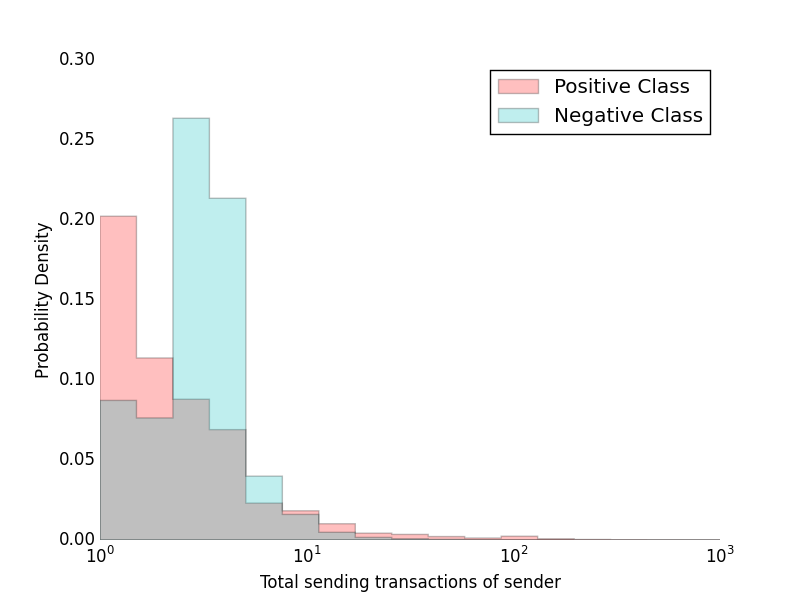
\includegraphics[width=0.5\textwidth]{figs/hist_out.png} & 
%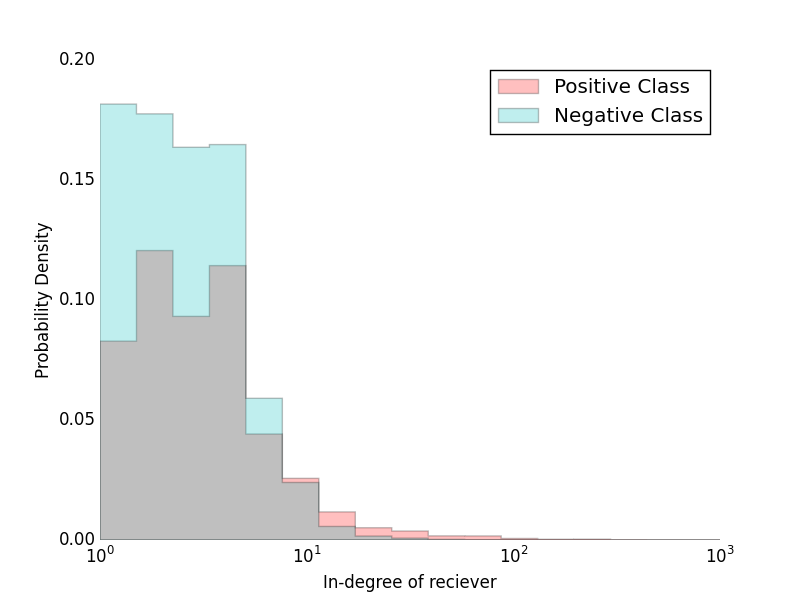
\includegraphics[width=0.4\textwidth]{figs/hist_in_deg.png} \\ 
%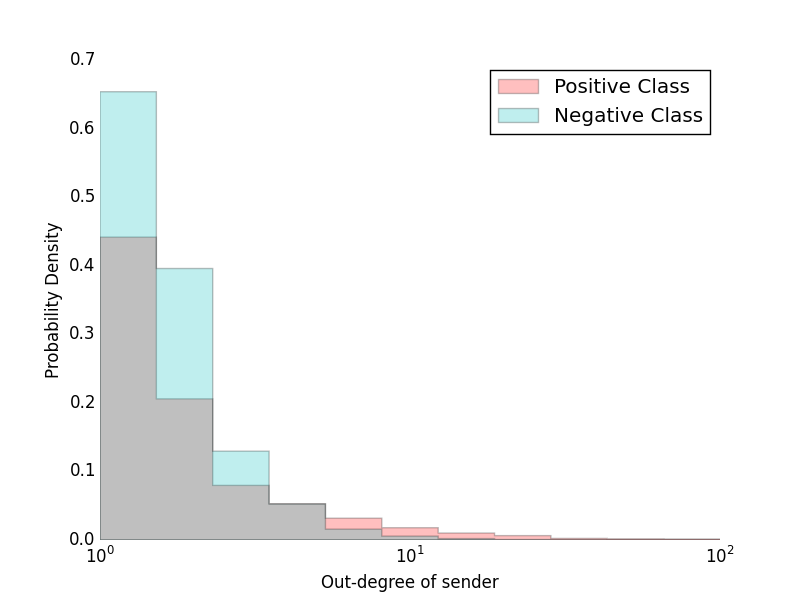
\includegraphics[width=0.4\textwidth]{figs/hist_out_deg.png} & 
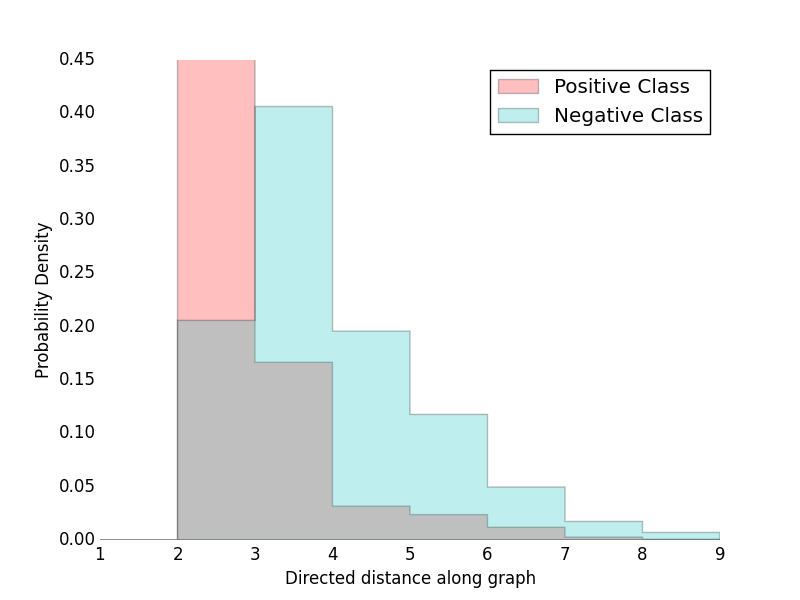
\includegraphics[width=0.5\textwidth]{figs/hist_dist.png}  
\end{tabular}
\label{fig:hist}
\end{figure}
Factorization (Decomposition) of a matrix involves numerically approximating it as a product of two or more matrices which contain feature information. One may set a small number of features to significantly reduce dimensionality of the component matrices, which is extremely useful since it extracts the strongest latent signals from otherwise noisy data and improves prediction accuracy. We test two decomposition models that support sparse matrices. 
\textbf{Singular Value Decomposition} (SVD) determines three component matrices. The outer two are unitary and are comprised of basis vectors. The central one is diagonal and contains the singular values.
\textbf{Non-negative Matrix Factorization} (NMF) assumes a non-negative input matrix, and determines two constituent matrices by minimizing the Frobenius norm \cite{scikit-learn}. Thus vectors are always superpositions of the components. These models are summarized in Figure~\ref{fig:matrix}.

\subsection{Graph Feature Extraction}
\begin{wrapfigure}{r}{5.6cm}
%\centering
 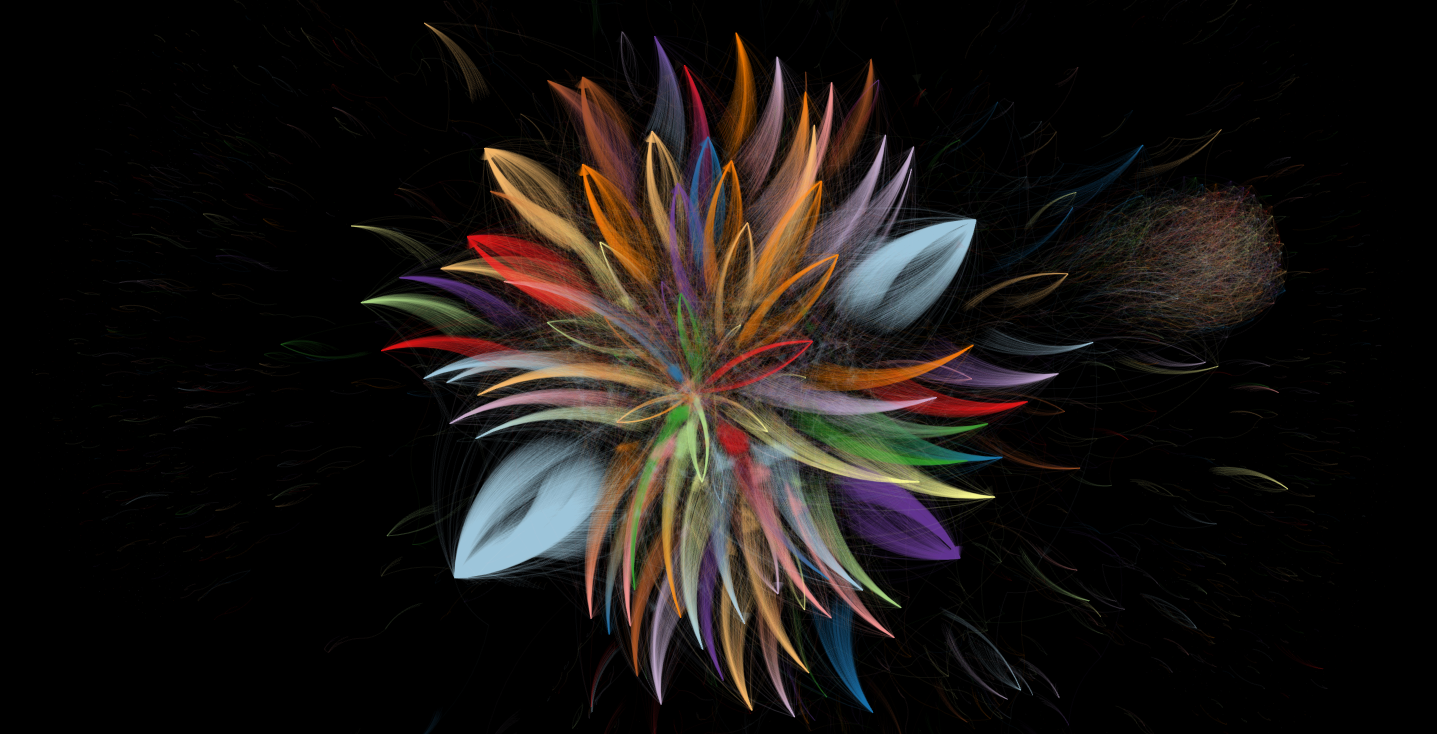
\includegraphics[trim={6cm 2cm 6cm 2cm},clip,width=5.6cm]{50000visualization.png}
\caption{Visualization of 50000 randomly selected transactions. The most active nodes are clearly visible. Connections among these addresses form the basis for our graph analysis.}
\label{fig:vis}
\end{wrapfigure}

An entirely separate approach to the data involved extraction of a number of features from the directed-graph representation of the blockchain.  Using the python graph-processing package NetworkX \cite{nx}, each transaction in the training data was modeled as a directed edge from the node representing sending address to the node of the receiver, with the number of transactions stored as an attribute of the edge.  A subset of the graph can be seen visualized in Figure~\ref{fig:vis}. A number of features were then extracted from this graph to simulate the two classes of address pairs: that is future transaction or no future transaction.

To simulate a pair in the no-transaction (negative) class, two random addresses were selected at random, repeating the selection if they already had a directed edge between them.  Then using the methods from NetworkX, the following features were compiled: out-degree of the sending address, in-degree of the receiving address, total number of transactions of each address, and the length of the shortest directed path between the two.  The positive class was simulated by selecting a transaction from the training list at random, and temporarily removing the directed edge from the graph, then computing the same features without the transaction in question, and re-adding the link before computing another pair.  Promisingly, histograms for these features tended to segregate the two classes noticably, as seen in Figure~\ref{fig:hist}.  These features were calculated for one hundred thousand random pairs, keeping the class-priors consistent with the inflated test data: 10\% positive and 90\% negative.  The same features calculated above were calculated for each pair of addresses in the test set.  


\subsubsection{Classification Methods}
Several models were trained on the binary classification task using the compiled feature vectors.  Given the low dimensionality of the feature space (5), and the apparent separation of the features seen in the histograms of Figure~\ref{fig:hist} we used three simple models:

\begin{itemize}
	\item \textbf{Random Forest}: Ensemble of decision-tree classifiers
	\item \textbf{Naive Bayes}: Three separate models, one using the 5 features and multinomial prior (MNB), another using the 5 features with Gaussian prior (GNB$_1$) and a third using the pairwise products of the five features to account for potential interactions between them, that is a total of 10 distinct features and a gaussian prior (GNB$_2$)
	\item \textbf{K Neighbors}: Optimized with $k=25$
\end{itemize}

Both the random forest and $k$ neighbors are particularly well-suited for low-dimensional feature spaces, and naive bayes is a good benchmark classifier for comparison.

\section{Results}

\subsection{Decomposition True Positive Rates}

Here we present the performance of our two matrix decomposition methods, SVD and NMF. We also compare them against 'Random,' in which the component matrices are randomly generated with elements in [0, 1]. Both of the decomposition methods perform much better than the random case, as summarized in Figure~\ref{fig:matrix}. NMF performs the best consistently, perhaps because of the non-negative assumption. It successfully identifies transactions at a true positive rate of 0.51, with an erroneous false positive rate of only 0.1. Both models however are far from optimal binary classification (a point at FPR = 0, TPR = 1). 
\begin{figure}[!h]

%\begin{table}[h]%
\begin{minipage}[b]{0.45\linewidth}
\centering

\begin{footnotesize}
\setlength{\tabcolsep}{4pt}
\renewcommand{\arraystretch}{2.85}
\begin{tabular}[b]{c c c c | c c c}
    \hline
    Name & Formula & $N_{comp}$ & tol & ROC & PR & TPR$_{{\rm FPR = } 0.1}$\\
    \hline
    {\it SVD} & $\mathbf{ X = USV}$ & 10 & $10^{-10}$ & 0.64 & 0.35 & 0.39 \\
    {\it NMF} & $\mathbf{ X = WH}$ & 20 & $10^{-10}$ & 0.74 & 0.37 & 0.51 \\
    {\it Random} & $\mathbf{ X = R^{1}R^{2}}$ & 10 & N/A & 0.50 & 0.10 & 0.10 \\
    \hline
\end{tabular}
\end{footnotesize}
%\caption{Table}

%\end{table}
\end{minipage}
\begin{minipage}[b]{0.8\linewidth}


\centering
  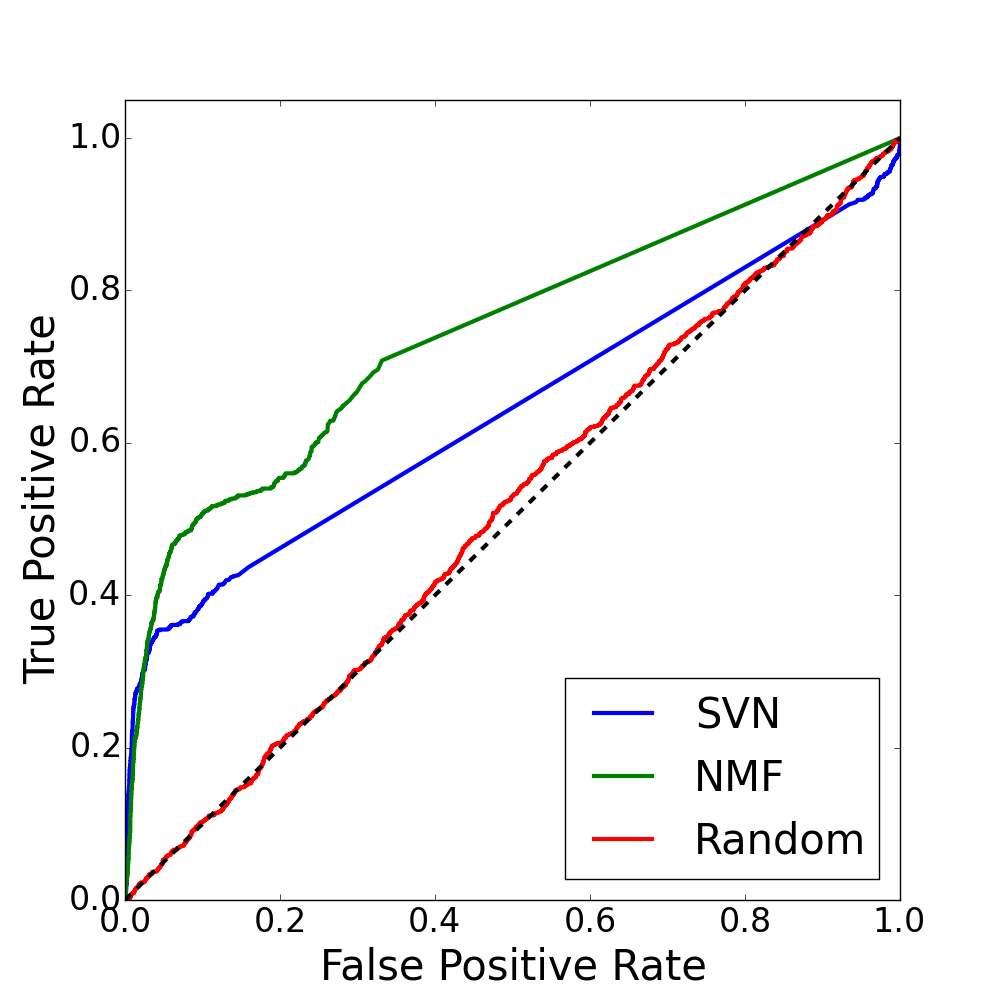
\includegraphics[width=0.45\textwidth]{ROC.png}
%  \caption{Receiver Operating Characteristic curves for each of the models.}
  \label{fig:roc}
\end{minipage}

\caption{Properties of matrix decomposition models including name, formulation, number of components (reduced dimension), and tolerance level. Also performance including ROC area, PR area, and true positive rate with at most 0.1 false positive rate. Parameters were chosen for a balance of run-time and accuracy.}
\label{fig:matrix}
\end{figure}

\subsection{Graph Classifier Performance}

\begin{figure}[!hbt]
\label{fig:classifiers}
\begin{tabular}{cc}
% actual figures
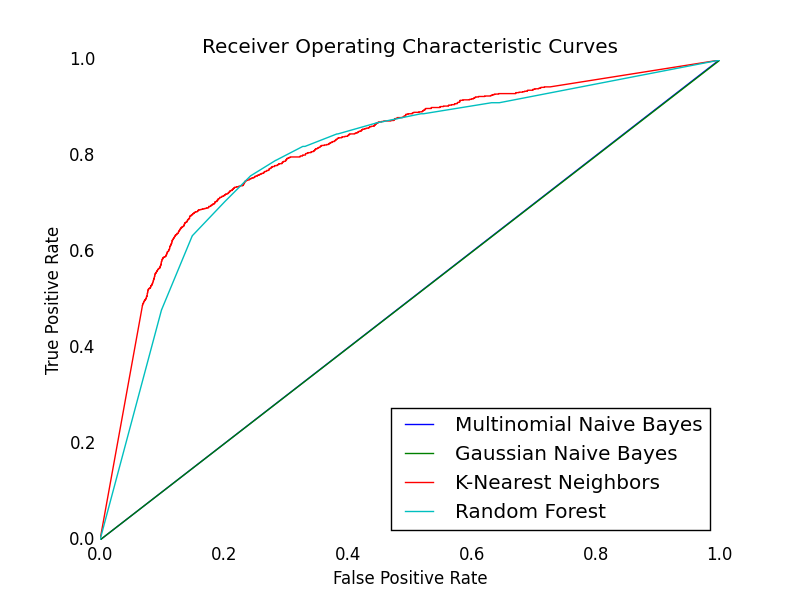
\includegraphics[width=0.5\textwidth]{figs/roc.png} &
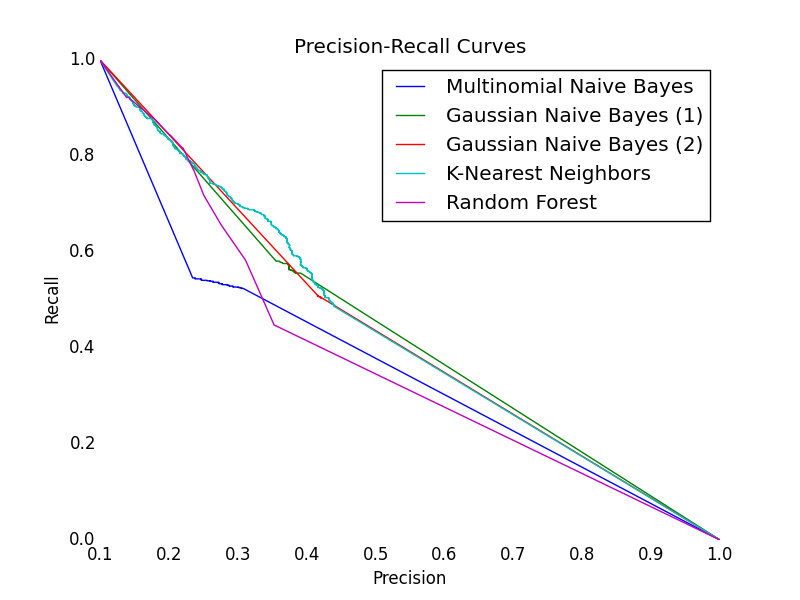
\includegraphics[width=0.5\textwidth]{figs/prc.png} \\
% table of areas
\multicolumn{2}{c}{\begin{tabular}{|l|c|c|c|c|c|}
\hline\textbf{Model}: &  GNB$_1$ & GNB$_2$ & MNB & K-Neighbors & Random Forest  \\ \hline
\textbf{ROC Area} & 0.737 & 0.716 & .690 & 0.818 & 0.801 \\ 
\textbf{P-R Area} & 0.492 & .487 &0.425 & 0.489 & 0.453  \\ 
\textbf{F1 Score} & 0.453 & .458 &0.357 &  0.377 & 0.369 \\ \hline 
\end{tabular}} 
\end{tabular}
\caption{Performance of binary classifiers trained on graph features.  Parameters were selected to maximize accuracy, and the class prior (when applicable) was set to reflect the frequency of each class in the test data.}
\end{figure}

The feature-based graph classifiers all performed better than the factorization methods.  All far surpassed the random matrix classifier described above.  Both $K$-Neighbors and the Random Forest classifiers achieved ROC area scores over 0.8, while the three Naive Bayes approaches had areas of about 0.7.  However, both Naive Bayes classifiers had a higher average accuracy score, corresponding to the area under the precision-recall curve, and a higher F1-Score, or ``balanced accuracy" than the $K$-Neighbors and Random Forest classifiers.  See Figure~\ref{fig:classifiers} for details.

\section{Discussion and Conclusion}
While the two approaches appear entirely distinct, they are attempting to capture the same idea in the data: is there a certain underlying structure in the transaction network such that left-out edges can be predicted?  The matrix in the factorization approaches is in fact the adjacency matrix of the graph, and reducing its dimensionality is an attempt to replace individual transactions with large scale patterns.  That is to say hubs on the graph will be compressed by the decomposition, and two elements of the same hub may be predicted to transact in the future, though they may not have in the past.  Were every transaction to be kept in the matrix, it would predict negative for every future pair that has not previously interacted, and so our approach was an exercise in keeping only enough information to capture the essence of the graph without reconstructing the entire thing.  This is quite a simple concept and proved to be very effective, but also due to its simplicity it was outperformed by the classifiers that took a more nuanced approach to the transaction graph. 

Gathering the training data for the classfiers as discussed in the methods was very computationally intensive, requiring about 6 hours for 100000 sender/receiver pairs.  However this step was only completed once, and models could subsequently be optimized with the gathered features.  These features, as shown in Figure~\ref{fig:hist} did tend to differ between classes, which makes intuitive sense.  Interpreting the models, it seemed that addresses closer to each other along the graph's edges were more likely to interact, and transactions were more likely to occur between already active senders and receivers.

With respect to model evaluation, the fact that $K$-Neighbors and Random Forest outperform all others in ROC area but have a low F1-score implies that they tend to overestimate the larger negative class.  The difference between the naive bayes priors is interesting, as the features given to GNB$_1$ and MNB are all positive integers and likely are described better by a multinomial distribution than Gaussian.  That said, with our $N$ quite large, the central limit theorem suggests our distributions are mostly Gaussian regardless.  In conclusion, we award our best performance to the GNB$_2$ model, which combines the advantages of allowing feature-interaction present in the $K$-Neighbors and Random Forest with the extreme adaptability of naive bayes classifiers in general.

For future research, increasing the number of features gathered from the graph, which was limited in this investigation by computational time constraints could likely find even more structure in the transaction network, and increasing the number of simulated transactions would only help every model.  

%\subsubsection*{Acknowledgments}
%We would like to thank the course staff and instructors for their invaluable %assistance.

\bibliography{ref}
\bibliographystyle{IEEEtran}
\ref{roc} Jesse Davis \& Mark Goadrich (2006), \emph{The Relationship Between Precision-Recall and ROC Curves.} Proceedings of the 23rd International Conference on Machine Learning.


\end{document}
